\documentclass[12pt,a4paper]{article}
\usepackage[margin=2cm]{geometry}
\usepackage{tikz}
\usetikzlibrary{arrows.meta,positioning,shapes.geometric,fit,calc,decorations.pathreplacing}
\usepackage{fancyhdr}
\usepackage{amsmath,amssymb}
\setlength{\headheight}{14.5pt}

\pagestyle{fancy}
\fancyhf{}
\rhead{Patent Drawings}
\lhead{Odeyemi O.I.}
\rfoot{Page \thepage}

\tikzset{
  blk/.style={draw, rectangle, minimum height=1cm, minimum width=3cm, align=center, font=\small, thick},
  sblk/.style={draw, rectangle, minimum height=0.7cm, minimum width=2.2cm, align=center, font=\scriptsize, thick},
  rblk/.style={draw, rounded corners=4pt, rectangle, minimum height=0.8cm, minimum width=2.5cm, align=center, font=\small, thick},
  diam/.style={draw, diamond, aspect=2, minimum width=1.5cm, align=center, font=\scriptsize, thick},
  arr/.style={-{Stealth[length=2.5mm]}, thick},
  darr/.style={-{Stealth[length=2.5mm]}, thick, dashed},
}

\begin{document}

\begin{center}
{\LARGE\bfseries DRAWINGS}\\[0.5em]
{\large State-Adaptive Compliance Enforcement System with\\
Multi-Spectrum Anomaly Detection and Failure-Mode Correction\\
for Decentralised Finance Networks}\\[0.5em]
{\normalsize Applicant: Odeyemi Olusegun Israel \quad Date: 4 March 2026}
\end{center}

\vspace{1em}

%% =========  FIGURE 1  =========
\begin{center}
\textbf{Figure 1 --- Overall Four-Layer System Architecture}
\end{center}

\begin{center}
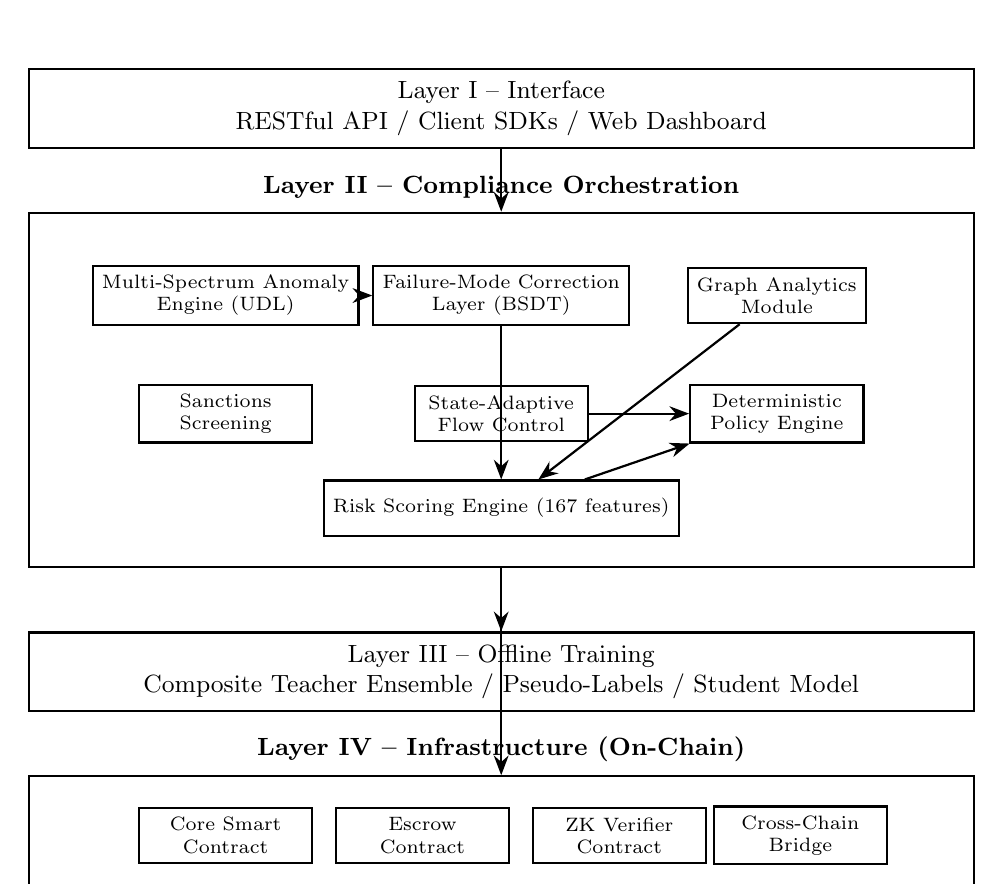
\begin{tikzpicture}[node distance=0.4cm]

% Layer I
\node[blk, minimum width=12cm] (api)
  {Layer I -- Interface\\RESTful API / Client SDKs / Web Dashboard};

% Layer II box
\node[blk, below=0.8cm of api, minimum width=12cm, minimum height=4.5cm] (l2bg) {};
\node[above=0.05cm of l2bg.north, font=\small\bfseries, anchor=south]
  {Layer II -- Compliance Orchestration};

\node[sblk] at ([yshift=1.2cm, xshift=-3.5cm]l2bg.center) (udl)
  {Multi-Spectrum Anomaly\\Engine (UDL)};
\node[sblk] at ([yshift=1.2cm]l2bg.center) (bsdt)
  {Failure-Mode Correction\\Layer (BSDT)};
\node[sblk] at ([yshift=1.2cm, xshift=3.5cm]l2bg.center) (graph)
  {Graph Analytics\\Module};

\node[sblk] at ([yshift=-0.3cm, xshift=-3.5cm]l2bg.center) (sanctions)
  {Sanctions\\Screening};
\node[sblk] at ([yshift=-0.3cm]l2bg.center) (af)
  {State-Adaptive\\Flow Control};
\node[sblk] at ([yshift=-0.3cm, xshift=3.5cm]l2bg.center) (policy)
  {Deterministic\\Policy Engine};

\node[sblk] at ([yshift=-1.5cm]l2bg.center) (risk)
  {Risk Scoring Engine (167 features)};

% Layer III
\node[blk, below=0.8cm of l2bg, minimum width=12cm] (l3)
  {Layer III -- Offline Training\\Composite Teacher Ensemble / Pseudo-Labels / Student Model};

% Layer IV
\node[blk, below=0.8cm of l3, minimum width=12cm, minimum height=1.5cm] (l4bg) {};
\node[above=0.05cm of l4bg.north, font=\small\bfseries, anchor=south]
  {Layer IV -- Infrastructure (On-Chain)};

\node[sblk] at ([xshift=-3.5cm]l4bg.center) (core) {Core Smart\\Contract};
\node[sblk] at ([xshift=-1cm]l4bg.center) (escrow) {Escrow\\Contract};
\node[sblk] at ([xshift=1.5cm]l4bg.center) (zkv) {ZK Verifier\\Contract};
\node[sblk] at ([xshift=3.8cm]l4bg.center) (bridge) {Cross-Chain\\Bridge};

% Arrows
\draw[arr] (api) -- (l2bg);
\draw[arr] (udl) -- (bsdt);
\draw[arr] (bsdt) -- (risk);
\draw[arr] (graph) -- (risk);
\draw[arr] (af) -- (policy);
\draw[arr] (risk) -- (policy);
\draw[arr] (l2bg) -- (l3);
\draw[arr] (l2bg) -- (l4bg);

\end{tikzpicture}
\end{center}

\newpage

%% =========  FIGURE 2  =========
\begin{center}
\textbf{Figure 2 --- Pre-Settlement Smart Contract Enforcement Workflow}
\end{center}

\begin{center}
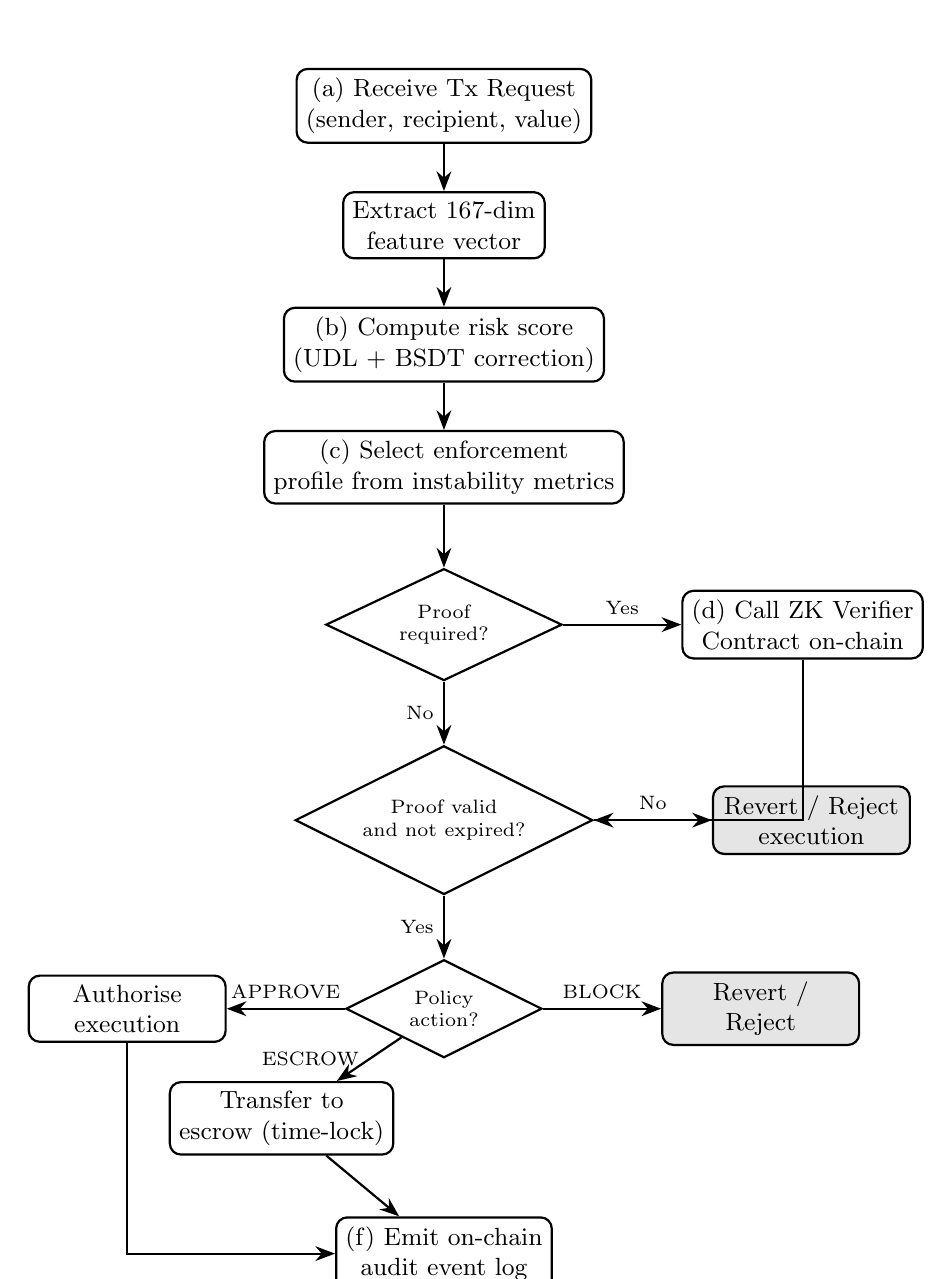
\begin{tikzpicture}[node distance=0.6cm]

\node[rblk] (rx) {(a) Receive Tx Request\\(sender, recipient, value)};
\node[rblk, below=of rx] (feat) {Extract 167-dim\\feature vector};
\node[rblk, below=of feat] (score) {(b) Compute risk score\\(UDL + BSDT correction)};
\node[rblk, below=of score] (profile) {(c) Select enforcement\\profile from instability metrics};

\node[diam, below=0.8cm of profile, minimum width=3cm] (proofq) {Proof\\required?};
\node[rblk, right=1.5cm of proofq] (verify) {(d) Call ZK Verifier\\Contract on-chain};

\node[diam, below=0.8cm of proofq] (proofok) {Proof valid\\and not expired?};
\node[rblk, right=1.5cm of proofok, fill=black!10] (revert1) {Revert / Reject\\execution};

\node[diam, below=0.8cm of proofok] (action) {Policy\\action?};
\node[rblk, left=1.5cm of action] (approve) {Authorise\\execution};
\node[rblk, below left=0.6cm and 0cm of action] (escrowact) {Transfer to\\escrow (time-lock)};
\node[rblk, right=1.5cm of action, fill=black!10] (block) {Revert /\\Reject};

\node[rblk, below=2cm of action] (audit) {(f) Emit on-chain\\audit event log};

\draw[arr] (rx) -- (feat);
\draw[arr] (feat) -- (score);
\draw[arr] (score) -- (profile);
\draw[arr] (profile) -- (proofq);
\draw[arr] (proofq) -- node[above,font=\scriptsize]{Yes} (verify);
\draw[arr] (proofq) -- node[left,font=\scriptsize]{No} (proofok);
\draw[arr] (verify) |- (proofok);
\draw[arr] (proofok) -- node[above,font=\scriptsize]{No} (revert1);
\draw[arr] (proofok) -- node[left,font=\scriptsize]{Yes} (action);
\draw[arr] (action) -- node[above,font=\scriptsize]{APPROVE} (approve);
\draw[arr] (action) -- node[left,font=\scriptsize]{ESCROW} (escrowact);
\draw[arr] (action) -- node[above,font=\scriptsize]{BLOCK} (block);
\draw[arr] (approve) |- (audit);
\draw[arr] (escrowact) -- (audit);

\end{tikzpicture}
\end{center}

\newpage

%% =========  FIGURE 3  =========
\begin{center}
\textbf{Figure 3 --- Spectrum Operators and Anomaly Tensor Construction}
\end{center}

\begin{center}
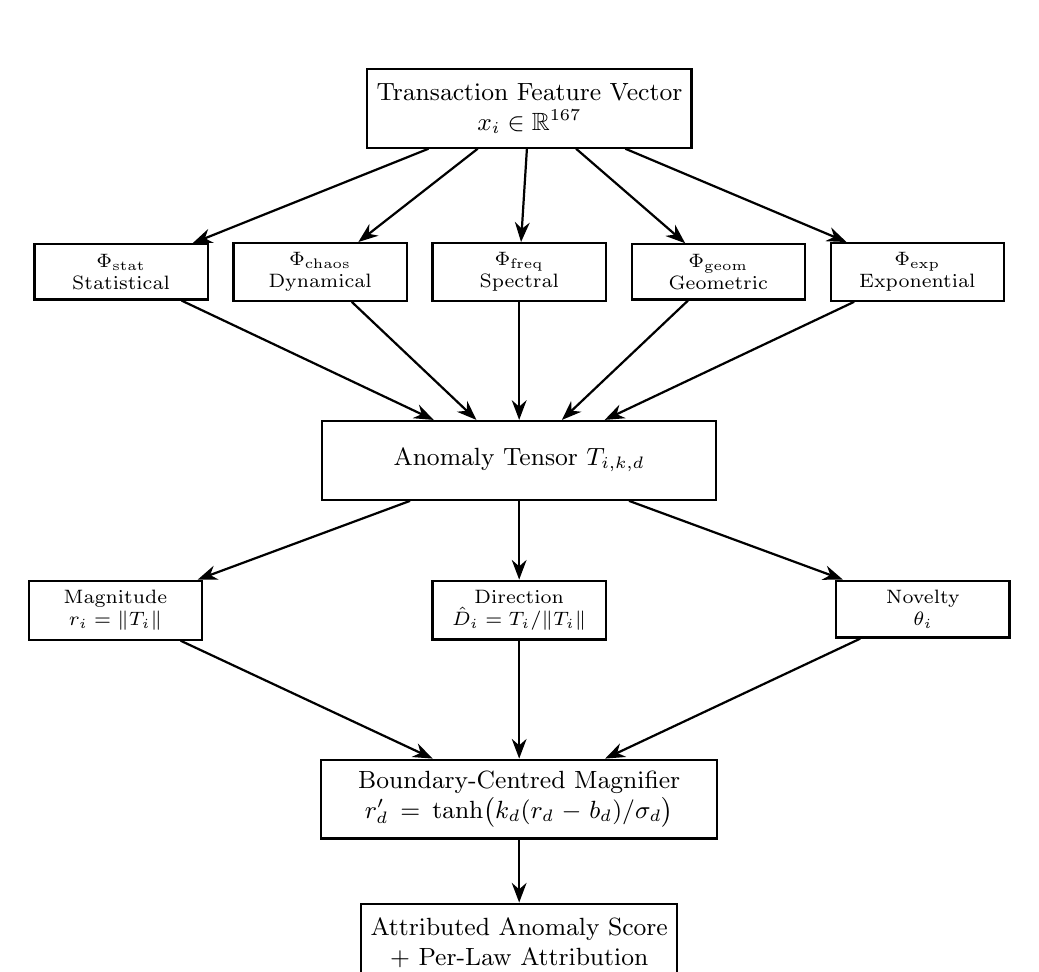
\begin{tikzpicture}[node distance=0.5cm]

\node[blk, minimum width=4cm] (input) {Transaction Feature Vector\\$x_i \in \mathbb{R}^{167}$};

\node[sblk, below left=1.2cm and 2cm of input] (stat) {$\Phi_{\mathrm{stat}}$\\Statistical};
\node[sblk, right=0.3cm of stat] (chaos) {$\Phi_{\mathrm{chaos}}$\\Dynamical};
\node[sblk, right=0.3cm of chaos] (freq) {$\Phi_{\mathrm{freq}}$\\Spectral};
\node[sblk, right=0.3cm of freq] (geom) {$\Phi_{\mathrm{geom}}$\\Geometric};
\node[sblk, right=0.3cm of geom] (expo) {$\Phi_{\mathrm{exp}}$\\Exponential};

\node[blk, below=1.5cm of freq, minimum width=5cm] (tensor) {Anomaly Tensor $T_{i,k,d}$};

\node[sblk, below left=1cm and 1.5cm of tensor] (mag) {Magnitude\\$r_i = \lVert T_i \rVert$};
\node[sblk, below=1cm of tensor] (dir) {Direction\\$\hat{D}_i = T_i / \lVert T_i \rVert$};
\node[sblk, below right=1cm and 1.5cm of tensor] (nov) {Novelty\\$\theta_i$};

\node[blk, below=1.5cm of dir, minimum width=5cm, text width=4.8cm] (magnifier)
  {Boundary-Centred Magnifier\\$r'_d = \tanh\bigl(k_d (r_d - b_d)/\sigma_d\bigr)$};

\node[blk, below=0.8cm of magnifier, minimum width=4cm] (out) {Attributed Anomaly Score\\+ Per-Law Attribution};

\foreach \op in {stat,chaos,freq,geom,expo} {
  \draw[arr] (input) -- (\op);
  \draw[arr] (\op) -- (tensor);
}
\draw[arr] (tensor) -- (mag);
\draw[arr] (tensor) -- (dir);
\draw[arr] (tensor) -- (nov);
\draw[arr] (mag) -- (magnifier);
\draw[arr] (dir) -- (magnifier);
\draw[arr] (nov) -- (magnifier);
\draw[arr] (magnifier) -- (out);

\end{tikzpicture}
\end{center}

\newpage

%% =========  FIGURE 4  =========
\begin{center}
\textbf{Figure 4 --- MDN Decomposition Schematic}
\end{center}

\begin{center}
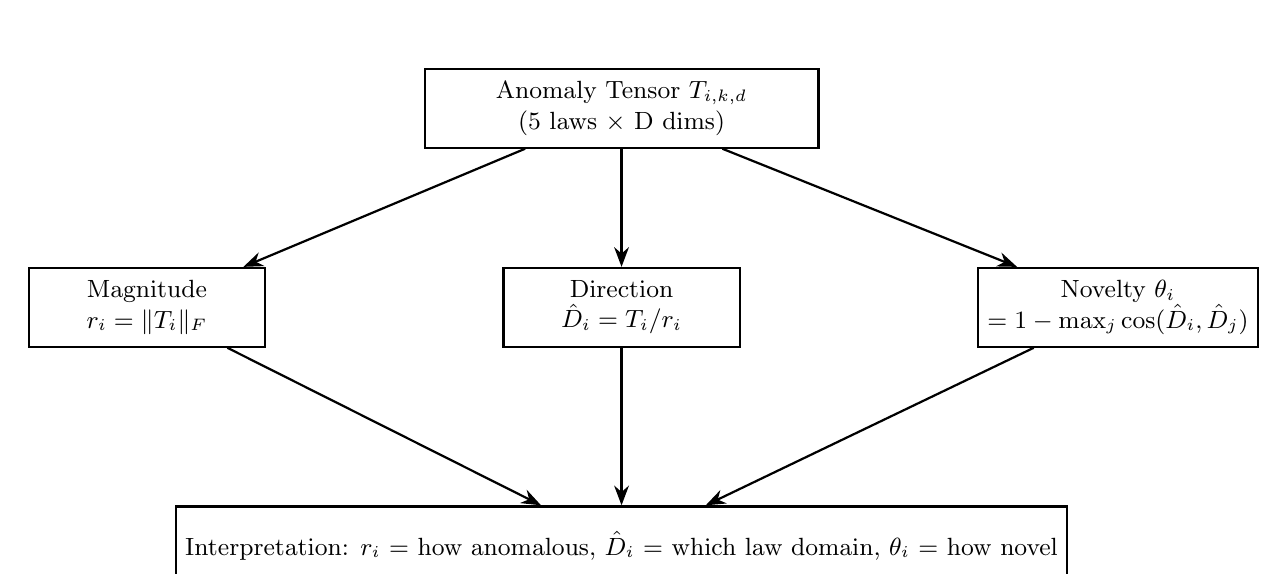
\begin{tikzpicture}[node distance=0.8cm]

\node[blk, minimum width=5cm] (tensor) {Anomaly Tensor $T_{i,k,d}$\\(5 laws $\times$ D dims)};

\node[blk, below left=1.5cm and 2cm of tensor, minimum width=3cm] (mag)
  {Magnitude\\$r_i = \lVert T_i \rVert_F$};
\node[blk, below=1.5cm of tensor, minimum width=3cm] (dir)
  {Direction\\$\hat{D}_i = T_i / r_i$};
\node[blk, below right=1.5cm and 2cm of tensor, minimum width=3cm] (nov)
  {Novelty $\theta_i$\\$= 1 - \max_j \cos(\hat{D}_i, \hat{D}_j)$};

\node[blk, below=2cm of dir, minimum width=8cm] (interp)
  {Interpretation: $r_i$ = how anomalous, $\hat{D}_i$ = which law domain, $\theta_i$ = how novel};

\draw[arr] (tensor) -- (mag);
\draw[arr] (tensor) -- (dir);
\draw[arr] (tensor) -- (nov);
\draw[arr] (mag) -- (interp);
\draw[arr] (dir) -- (interp);
\draw[arr] (nov) -- (interp);

\end{tikzpicture}
\end{center}

\newpage

%% =========  FIGURE 5  =========
\begin{center}
\textbf{Figure 5 --- Four-Component BSDT Failure-Mode Decomposition}
\end{center}

\begin{center}
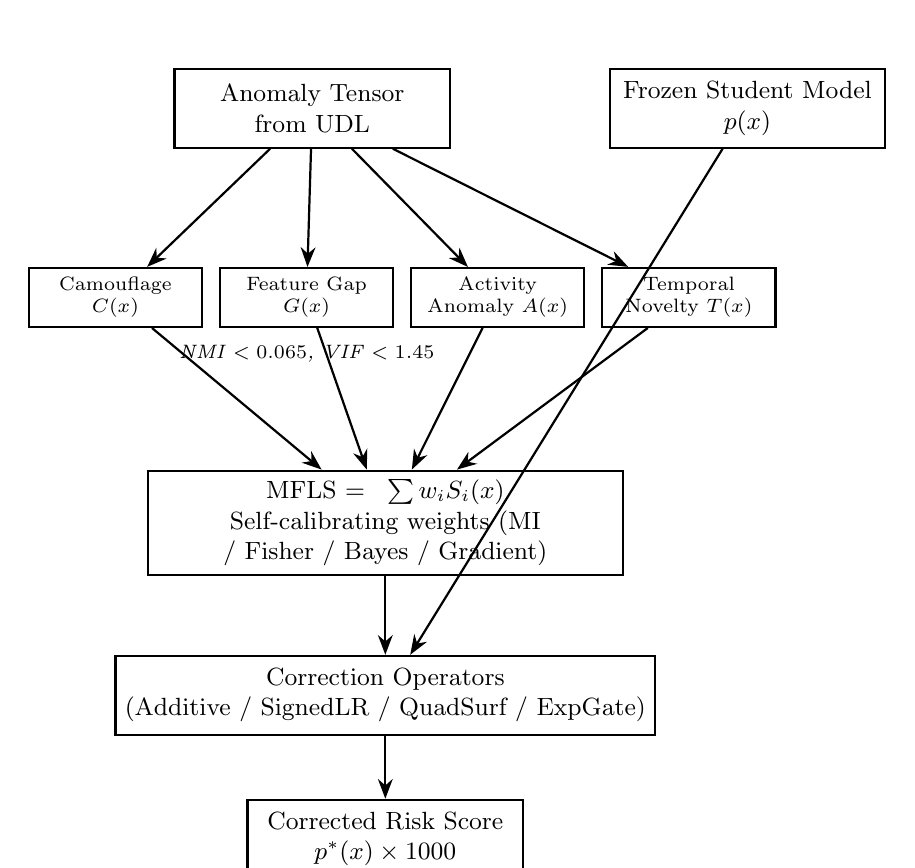
\begin{tikzpicture}[node distance=0.5cm]

\node[blk, minimum width=3.5cm] (tensor) {Anomaly Tensor\\from UDL};
\node[blk, right=2cm of tensor, minimum width=3.5cm] (frozen) {Frozen Student Model\\$p(x)$};

\node[sblk, below=1.5cm of tensor, xshift=-2.5cm] (C) {Camouflage\\$C(x)$};
\node[sblk, right=0.2cm of C] (G) {Feature Gap\\$G(x)$};
\node[sblk, right=0.2cm of G] (A) {Activity\\Anomaly $A(x)$};
\node[sblk, right=0.2cm of A] (T) {Temporal\\Novelty $T(x)$};

\node[below=0.1cm of G, font=\scriptsize\itshape] {NMI $< 0.065$, VIF $< 1.45$};

\node[blk, below=1.8cm of G, xshift=1cm, minimum width=6cm, text width=5.8cm] (mfls)
  {MFLS $= \sum w_i S_i(x)$\\Self-calibrating weights (MI / Fisher / Bayes / Gradient)};

\node[blk, below=1cm of mfls, minimum width=5cm] (corr)
  {Correction Operators\\(Additive / SignedLR / QuadSurf / ExpGate)};

\node[blk, below=0.8cm of corr, minimum width=3.5cm] (pstar)
  {Corrected Risk Score\\$p^*(x) \times 1000$};

\draw[arr] (tensor) -- (C);
\draw[arr] (tensor) -- (G);
\draw[arr] (tensor) -- (A);
\draw[arr] (tensor) -- (T);
\draw[arr] (frozen) -- (corr);
\draw[arr] (C) -- (mfls);
\draw[arr] (G) -- (mfls);
\draw[arr] (A) -- (mfls);
\draw[arr] (T) -- (mfls);
\draw[arr] (mfls) -- (corr);
\draw[arr] (corr) -- (pstar);

\end{tikzpicture}
\end{center}

\newpage

%% =========  FIGURE 6  =========
\begin{center}
\textbf{Figure 6 --- Correction Operator Pipeline Flow}
\end{center}

\begin{center}
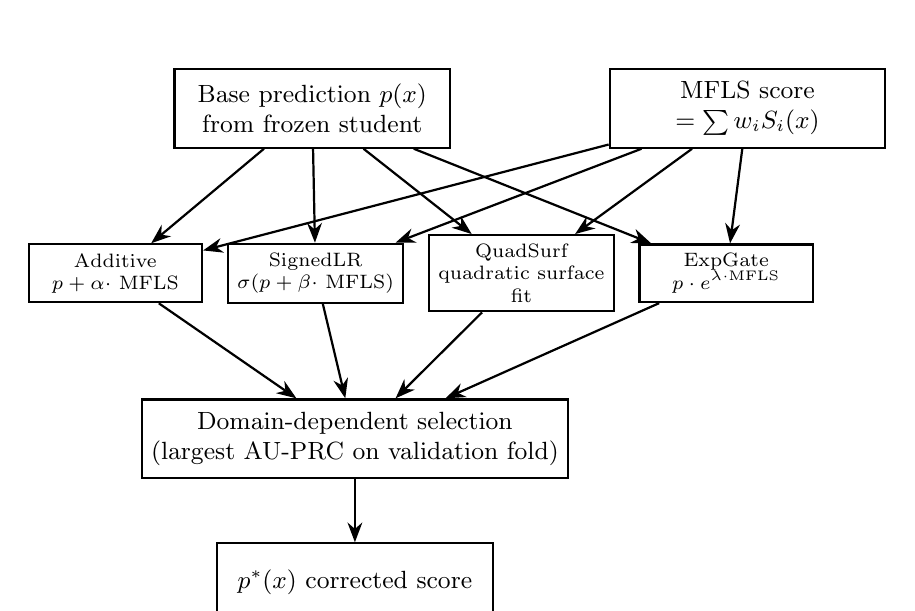
\begin{tikzpicture}[node distance=0.7cm]

\node[blk, minimum width=3.5cm] (base) {Base prediction $p(x)$\\from frozen student};
\node[blk, minimum width=3.5cm, right=2cm of base] (mfls) {MFLS score\\$= \sum w_i S_i(x)$};

\node[sblk, below=1.2cm of base, xshift=-2.5cm] (add) {Additive\\$p + \alpha \cdot$ MFLS};
\node[sblk, right=0.3cm of add] (slr) {SignedLR\\$\sigma(p + \beta \cdot$ MFLS$)$};
\node[sblk, right=0.3cm of slr] (quad) {QuadSurf\\quadratic surface\\fit};
\node[sblk, right=0.3cm of quad] (expg) {ExpGate\\$p \cdot e^{\lambda \cdot \mathrm{MFLS}}$};

\node[blk, below=1.2cm of slr, xshift=0.5cm, minimum width=5cm] (sel)
  {Domain-dependent selection\\(largest AU-PRC on validation fold)};

\node[blk, below=0.8cm of sel, minimum width=3.5cm] (out) {$p^*(x)$ corrected score};

\draw[arr] (base) -- (add);
\draw[arr] (base) -- (slr);
\draw[arr] (base) -- (quad);
\draw[arr] (base) -- (expg);
\draw[arr] (mfls) -- (add);
\draw[arr] (mfls) -- (slr);
\draw[arr] (mfls) -- (quad);
\draw[arr] (mfls) -- (expg);
\draw[arr] (add) -- (sel);
\draw[arr] (slr) -- (sel);
\draw[arr] (quad) -- (sel);
\draw[arr] (expg) -- (sel);
\draw[arr] (sel) -- (out);

\end{tikzpicture}
\end{center}

\newpage

%% =========  FIGURE 7  =========
\begin{center}
\textbf{Figure 7 --- Composite Teacher Weak Supervision Pipeline}
\end{center}

\begin{center}
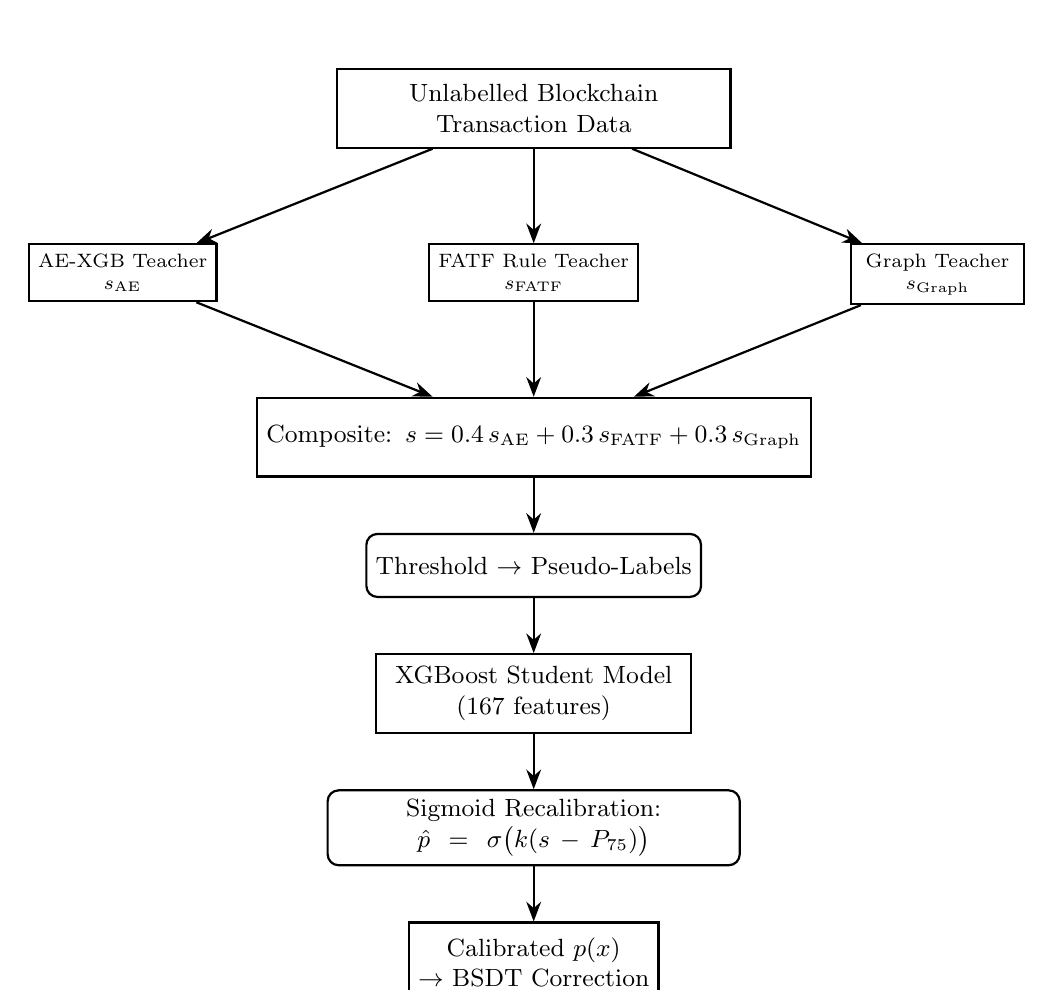
\begin{tikzpicture}[node distance=0.6cm]

\node[blk, minimum width=5cm] (data) {Unlabelled Blockchain\\Transaction Data};

\node[sblk, below left=1.2cm and 1.5cm of data] (ae) {AE-XGB Teacher\\$s_{\mathrm{AE}}$};
\node[sblk, below=1.2cm of data] (fatf) {FATF Rule Teacher\\$s_{\mathrm{FATF}}$};
\node[sblk, below right=1.2cm and 1.5cm of data] (gra) {Graph Teacher\\$s_{\mathrm{Graph}}$};

\node[blk, below=1.2cm of fatf, minimum width=7cm, text width=6.8cm] (comp)
  {Composite: $s = 0.4\, s_{\mathrm{AE}} + 0.3\, s_{\mathrm{FATF}} + 0.3\, s_{\mathrm{Graph}}$};

\node[rblk, below=0.7cm of comp] (pseudo) {Threshold $\to$ Pseudo-Labels};

\node[blk, below=0.7cm of pseudo, minimum width=4cm] (student) {XGBoost Student Model\\(167 features)};

\node[rblk, below=0.7cm of student, text width=5cm] (calib)
  {Sigmoid Recalibration:\\$\hat{p} = \sigma\bigl(k(s - P_{75})\bigr)$};

\node[blk, below=0.7cm of calib, minimum width=3cm] (out) {Calibrated $p(x)$\\$\to$ BSDT Correction};

\draw[arr] (data) -- (ae);
\draw[arr] (data) -- (fatf);
\draw[arr] (data) -- (gra);
\draw[arr] (ae) -- (comp);
\draw[arr] (fatf) -- (comp);
\draw[arr] (gra) -- (comp);
\draw[arr] (comp) -- (pseudo);
\draw[arr] (pseudo) -- (student);
\draw[arr] (student) -- (calib);
\draw[arr] (calib) -- (out);

\end{tikzpicture}
\end{center}

\newpage

%% =========  FIGURE 8  =========
\begin{center}
\textbf{Figure 8 --- Compliance Decision Matrix with Enforcement Profiles}
\end{center}

\begin{center}
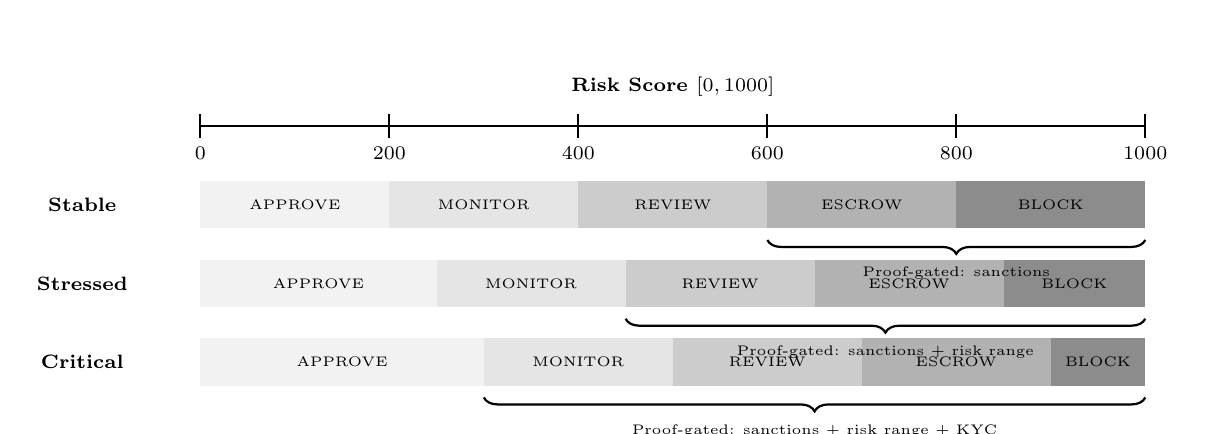
\begin{tikzpicture}[node distance=0.3cm]

% Score bar
\draw[thick] (0,0) -- (12,0);
\foreach \x/\lab in {0/0, 2.4/200, 4.8/400, 7.2/600, 9.6/800, 12/1000} {
  \draw[thick] (\x,-0.15) -- (\x,0.15);
  \node[below, font=\scriptsize] at (\x,-0.15) {\lab};
}
\node[above, font=\scriptsize\bfseries] at (6,0.25) {Risk Score $[0,1000]$};

% Stable
\node[font=\scriptsize\bfseries] at (-1.5, -1) {Stable};
\fill[black!5] (0,-0.7) rectangle (2.4,-1.3);
\fill[black!10] (2.4,-0.7) rectangle (4.8,-1.3);
\fill[black!20] (4.8,-0.7) rectangle (7.2,-1.3);
\fill[black!30] (7.2,-0.7) rectangle (9.6,-1.3);
\fill[black!45] (9.6,-0.7) rectangle (12,-1.3);
\node[font=\tiny] at (1.2,-1) {APPROVE};
\node[font=\tiny] at (3.6,-1) {MONITOR};
\node[font=\tiny] at (6,-1) {REVIEW};
\node[font=\tiny] at (8.4,-1) {ESCROW};
\node[font=\tiny] at (10.8,-1) {BLOCK};

% Stressed
\node[font=\scriptsize\bfseries] at (-1.5, -2) {Stressed};
\fill[black!5] (0,-1.7) rectangle (3,-2.3);
\fill[black!10] (3,-1.7) rectangle (5.4,-2.3);
\fill[black!20] (5.4,-1.7) rectangle (7.8,-2.3);
\fill[black!30] (7.8,-1.7) rectangle (10.2,-2.3);
\fill[black!45] (10.2,-1.7) rectangle (12,-2.3);
\node[font=\tiny] at (1.5,-2) {APPROVE};
\node[font=\tiny] at (4.2,-2) {MONITOR};
\node[font=\tiny] at (6.6,-2) {REVIEW};
\node[font=\tiny] at (9,-2) {ESCROW};
\node[font=\tiny] at (11.1,-2) {BLOCK};

% Critical
\node[font=\scriptsize\bfseries] at (-1.5, -3) {Critical};
\fill[black!5] (0,-2.7) rectangle (3.6,-3.3);
\fill[black!10] (3.6,-2.7) rectangle (6,-3.3);
\fill[black!20] (6,-2.7) rectangle (8.4,-3.3);
\fill[black!30] (8.4,-2.7) rectangle (10.8,-3.3);
\fill[black!45] (10.8,-2.7) rectangle (12,-3.3);
\node[font=\tiny] at (1.8,-3) {APPROVE};
\node[font=\tiny] at (4.8,-3) {MONITOR};
\node[font=\tiny] at (7.2,-3) {REVIEW};
\node[font=\tiny] at (9.6,-3) {ESCROW};
\node[font=\tiny] at (11.4,-3) {BLOCK};

% Proof-gating braces
\draw[thick, decorate, decoration={brace, amplitude=5pt, mirror}]
  (7.2, -1.45) -- (12, -1.45)
  node[midway, below=6pt, font=\tiny] {Proof-gated: sanctions};

\draw[thick, decorate, decoration={brace, amplitude=5pt, mirror}]
  (5.4, -2.45) -- (12, -2.45)
  node[midway, below=6pt, font=\tiny] {Proof-gated: sanctions + risk range};

\draw[thick, decorate, decoration={brace, amplitude=5pt, mirror}]
  (3.6, -3.45) -- (12, -3.45)
  node[midway, below=6pt, font=\tiny] {Proof-gated: sanctions + risk range + KYC};

\end{tikzpicture}
\end{center}

\newpage

%% =========  FIGURE 9  =========
\begin{center}
\textbf{Figure 9 --- zkNAF Circuit and On-Chain Verification Flow}
\end{center}

\begin{center}
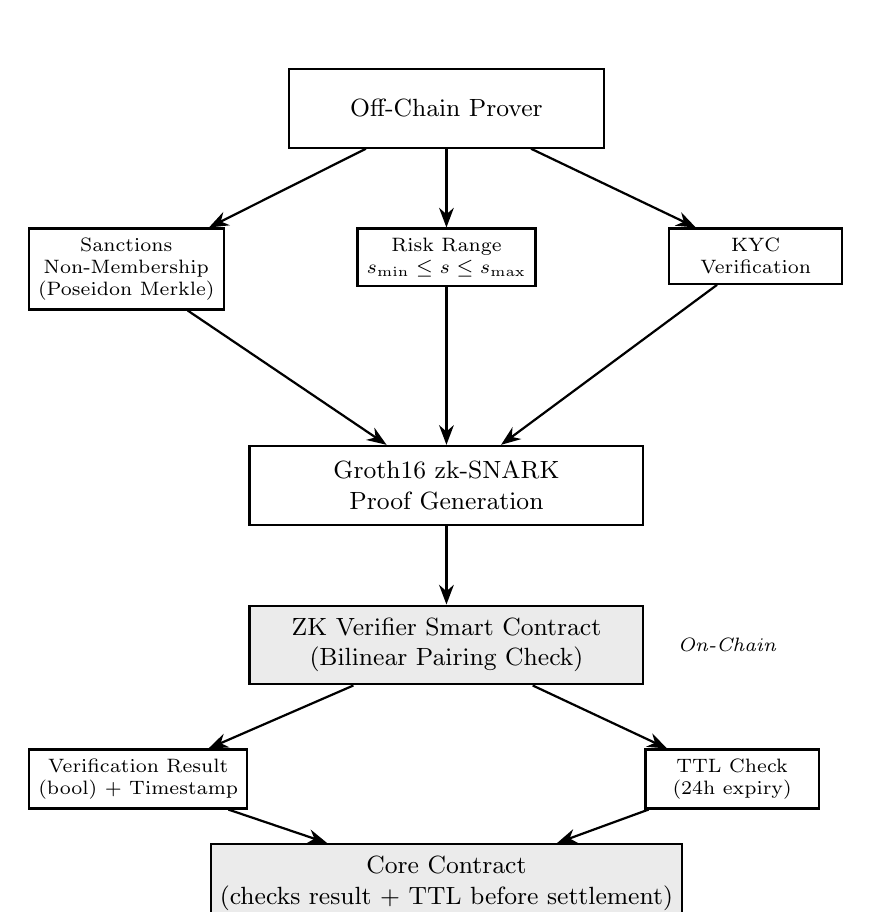
\begin{tikzpicture}[node distance=0.5cm]

\node[blk, minimum width=4cm] (prover) {Off-Chain Prover};

\node[sblk, below left=1cm and 0.8cm of prover] (sanc) {Sanctions\\Non-Membership\\(Poseidon Merkle)};
\node[sblk, below=1cm of prover] (range) {Risk Range\\$s_{\min} \leq s \leq s_{\max}$};
\node[sblk, below right=1cm and 0.8cm of prover] (kyc) {KYC\\Verification};

\node[blk, below=2cm of range, minimum width=5cm] (groth) {Groth16 zk-SNARK\\Proof Generation};

\node[blk, below=1cm of groth, minimum width=5cm, fill=black!8] (verifier)
  {ZK Verifier Smart Contract\\(Bilinear Pairing Check)};

\node[sblk, below left=0.8cm and 0cm of verifier] (result) {Verification Result\\(bool) + Timestamp};
\node[sblk, below right=0.8cm and 0cm of verifier] (ttl) {TTL Check\\(24h expiry)};

\node[blk, below=2cm of verifier, minimum width=5cm, fill=black!8] (coreC)
  {Core Contract\\(checks result + TTL before settlement)};

\draw[arr] (prover) -- (sanc);
\draw[arr] (prover) -- (range);
\draw[arr] (prover) -- (kyc);
\draw[arr] (sanc) -- (groth);
\draw[arr] (range) -- (groth);
\draw[arr] (kyc) -- (groth);
\draw[arr] (groth) -- (verifier);
\draw[arr] (verifier) -- (result);
\draw[arr] (verifier) -- (ttl);
\draw[arr] (result) -- (coreC);
\draw[arr] (ttl) -- (coreC);

\node[right=0.3cm of verifier, font=\scriptsize\itshape] {On-Chain};

\end{tikzpicture}
\end{center}

\newpage

%% =========  FIGURE 10  =========
\begin{center}
\textbf{Figure 10 --- GravityEngine N-Body Interaction Model}
\end{center}

\begin{center}
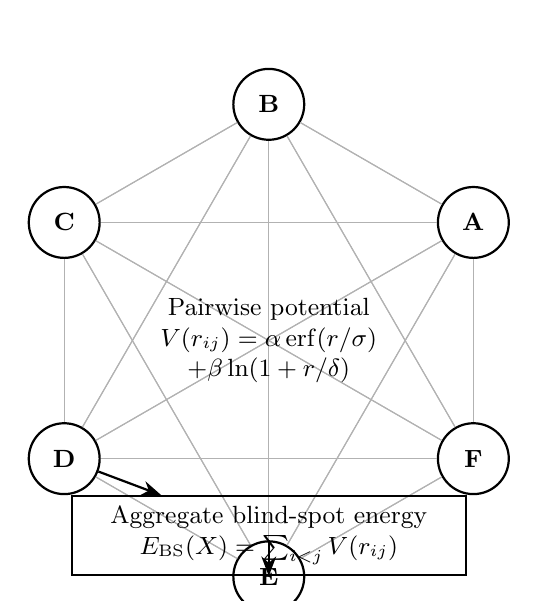
\begin{tikzpicture}

% Institutions as circles
\foreach \ang/\lab/\nm in {
  30/A/a, 90/B/b, 150/C/c, 210/D/d, 270/E/e, 330/F/f} {
  \node[draw, circle, thick, minimum size=0.9cm, font=\small\bfseries]
    (\nm) at (\ang:3cm) {\lab};
}

% Pairwise interaction lines
\foreach \i in {a,b,c,d,e,f} {
  \foreach \j in {a,b,c,d,e,f} {
    \ifx\i\j\else
      \draw[thin, black!30] (\i) -- (\j);
    \fi
  }
}

% Center label
\node[font=\small, align=center] at (0,0)
  {Pairwise potential\\$V(r_{ij}) = \alpha\,\mathrm{erf}(r/\sigma)$\\$+ \beta\ln(1+r/\delta)$};

% Blind-spot energy annotation
\node[blk, below=4.5cm of b, minimum width=5cm] (bse)
  {Aggregate blind-spot energy\\$E_{\mathrm{BS}}(X) = \sum_{i<j} V(r_{ij})$};

\draw[arr] (d) -- (bse);
\draw[arr] (e) -- (bse);

\end{tikzpicture}
\end{center}

\newpage

%% =========  FIGURE 11  =========
\begin{center}
\textbf{Figure 11 --- Critical Manifold and Enforcement Profile Regions}
\end{center}

\begin{center}
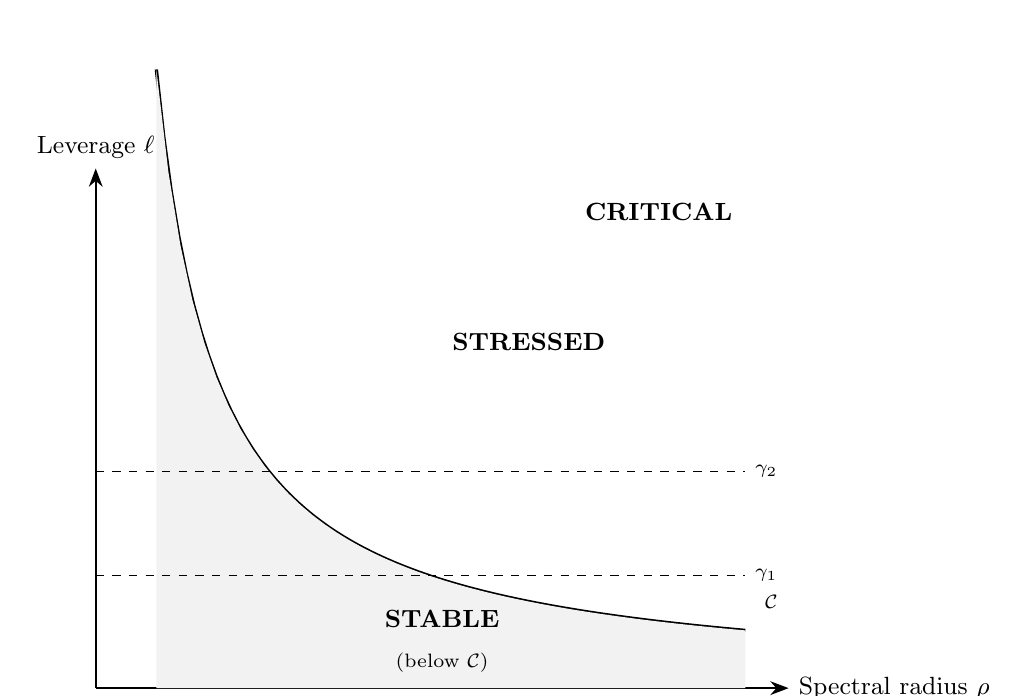
\begin{tikzpicture}[scale=1.1]

% Axes
\draw[thick, -{Stealth}] (0,0) -- (8,0) node[right, font=\small] {Spectral radius $\rho$};
\draw[thick, -{Stealth}] (0,0) -- (0,6) node[above, font=\small] {Leverage $\ell$};

% Critical manifold curve
\draw[very thick, domain=0.7:7.5, samples=80]
  plot (\x, {5/\x});
\node[font=\scriptsize] at (7.8, 1) {$\mathcal{C}$};

% Stable region shading
\fill[black!5, domain=0.7:7.5, samples=50]
  (0.7,0) -- plot (\x, {5/\x}) -- (7.5,0) -- cycle;

% Region labels
\node[font=\small\bfseries] at (4, 0.8) {STABLE};
\node[font=\scriptsize] at (4, 0.3) {(below $\mathcal{C}$)};

\node[font=\small\bfseries] at (5, 4) {STRESSED};

\node[font=\small\bfseries] at (6.5, 5.5) {CRITICAL};

% Threshold lines
\draw[dashed, thin] (0,2.5) -- (7.5,2.5) node[right, font=\scriptsize] {$\gamma_2$};
\draw[dashed, thin] (0,1.3) -- (7.5,1.3) node[right, font=\scriptsize] {$\gamma_1$};

\end{tikzpicture}
\end{center}

\newpage

%% =========  FIGURE 12  =========
\begin{center}
\textbf{Figure 12 --- State-Adaptive Transaction Flow Control Module}
\end{center}

\begin{center}
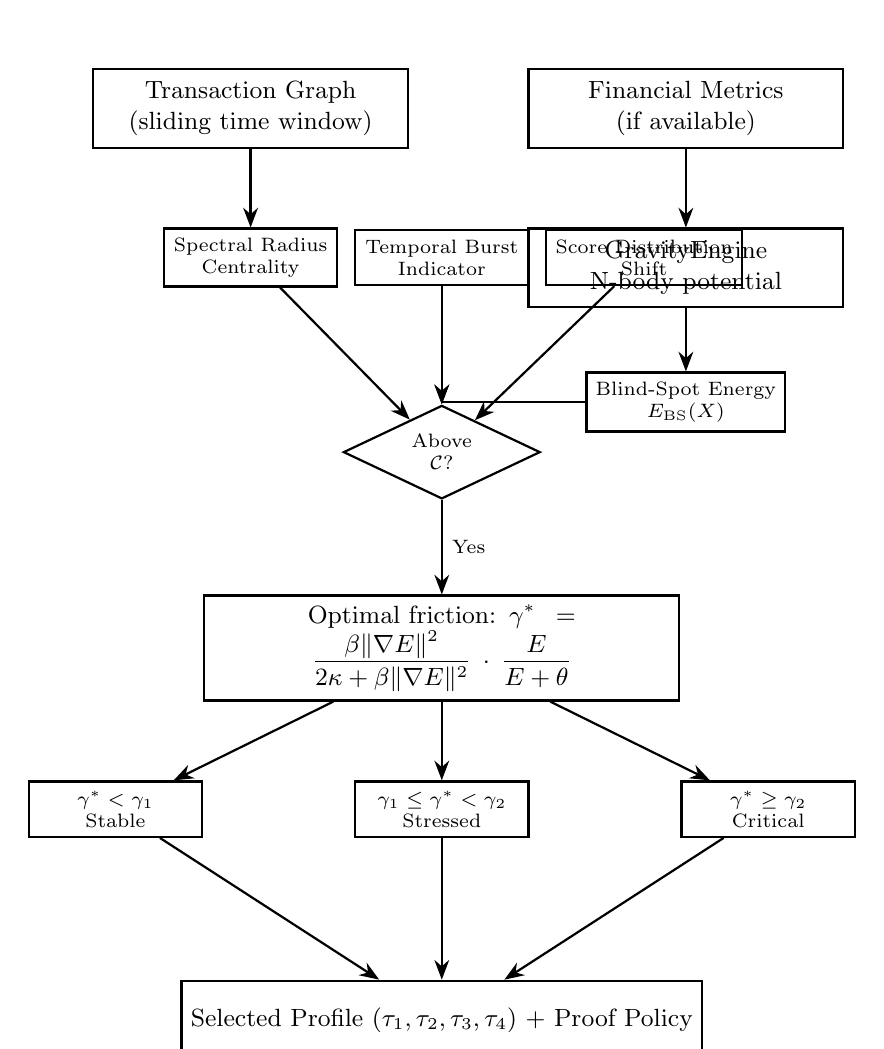
\begin{tikzpicture}[node distance=0.5cm]

\node[blk, minimum width=4cm] (txgraph) {Transaction Graph\\(sliding time window)};
\node[blk, right=1.5cm of txgraph, minimum width=4cm] (instdata) {Financial Metrics\\(if available)};

\node[sblk, below=1cm of txgraph] (spectral) {Spectral Radius\\Centrality};
\node[sblk, right=0.2cm of spectral] (burst) {Temporal Burst\\Indicator};
\node[sblk, right=0.2cm of burst] (shift) {Score Distribution\\Shift};

\node[blk, below=1cm of instdata, minimum width=4cm] (gravity) {GravityEngine\\N-body potential};

\node[sblk, below=0.8cm of gravity] (bseF) {Blind-Spot Energy\\$E_{\mathrm{BS}}(X)$};

\node[diam, below=1.5cm of burst, minimum width=2.5cm] (crit) {Above\\$\mathcal{C}$?};

\node[blk, below=1.2cm of crit, minimum width=6cm, text width=5.8cm] (gamma)
  {Optimal friction: $\gamma^* = \dfrac{\beta \lVert \nabla E \rVert^2}{2\kappa + \beta \lVert \nabla E \rVert^2} \cdot \dfrac{E}{E+\theta}$};

\node[sblk, below left=1cm and 0cm of gamma] (stable) {$\gamma^* < \gamma_1$\\Stable};
\node[sblk, below=1cm of gamma] (stressed) {$\gamma_1 \leq \gamma^* < \gamma_2$\\Stressed};
\node[sblk, below right=1cm and 0cm of gamma] (critical) {$\gamma^* \geq \gamma_2$\\Critical};

\node[blk, below=1.8cm of stressed, minimum width=6cm] (output)
  {Selected Profile $(\tau_1,\tau_2,\tau_3,\tau_4)$ + Proof Policy};

\draw[arr] (txgraph) -- (spectral);
\draw[arr] (instdata) -- (gravity);
\draw[arr] (gravity) -- (bseF);
\draw[arr] (spectral) -- (crit);
\draw[arr] (burst) -- (crit);
\draw[arr] (shift) -- (crit);
\draw[arr] (bseF) -| (crit);
\draw[arr] (crit) -- node[right,font=\scriptsize]{Yes} (gamma);
\draw[arr] (gamma) -- (stable);
\draw[arr] (gamma) -- (stressed);
\draw[arr] (gamma) -- (critical);
\draw[arr] (stable) -- (output);
\draw[arr] (stressed) -- (output);
\draw[arr] (critical) -- (output);

\end{tikzpicture}
\end{center}

\newpage

%% =========  FIGURE 13  =========
\begin{center}
\textbf{Figure 13 --- Navier--Stokes Analogy Schematic}
\end{center}

\begin{center}
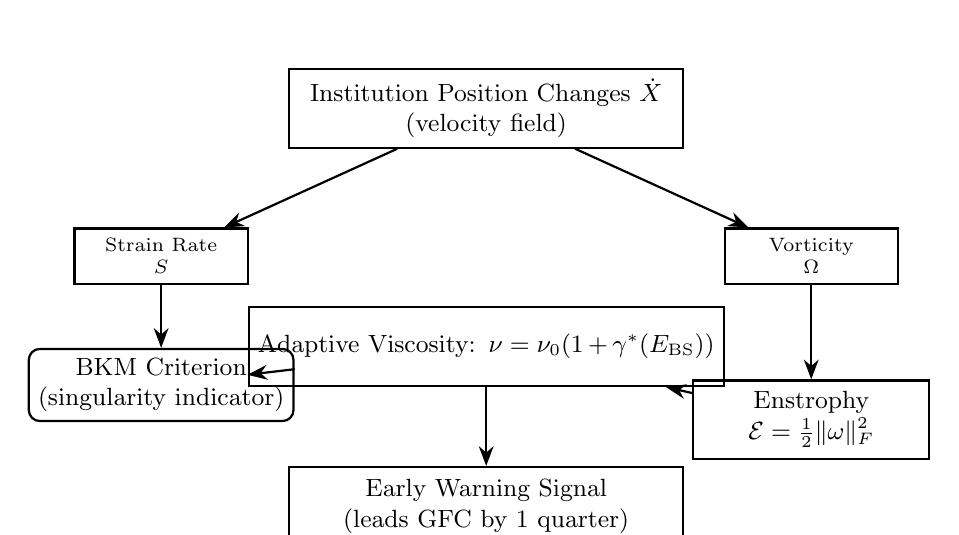
\begin{tikzpicture}[node distance=0.6cm]

\node[blk, minimum width=5cm] (pos) {Institution Position Changes $\dot{X}$\\(velocity field)};

\node[sblk, below left=1cm and 0.5cm of pos] (strain) {Strain Rate\\$S$};
\node[sblk, below right=1cm and 0.5cm of pos] (vort) {Vorticity\\$\Omega$};

\node[blk, below=1.2cm of vort, minimum width=3cm] (enst) {Enstrophy\\$\mathcal{E} = \tfrac{1}{2}\lVert\omega\rVert_F^2$};

\node[rblk, below=0.8cm of strain] (bkm) {BKM Criterion\\(singularity indicator)};

\node[blk, below=2cm of pos, minimum width=6cm, text width=5.8cm] (visc)
  {Adaptive Viscosity: $\nu = \nu_0(1 + \gamma^*(E_{\mathrm{BS}}))$};

\node[blk, below=1cm of visc, minimum width=5cm] (ewarn) {Early Warning Signal\\(leads GFC by 1 quarter)};

\draw[arr] (pos) -- (strain);
\draw[arr] (pos) -- (vort);
\draw[arr] (vort) -- (enst);
\draw[arr] (strain) -- (bkm);
\draw[arr] (enst) -- (visc);
\draw[arr] (bkm) -- (visc);
\draw[arr] (visc) -- (ewarn);

\end{tikzpicture}
\end{center}

\newpage

%% =========  FIGURE 14  =========
\begin{center}
\textbf{Figure 14 --- Minsky Regime Classification Diagram}
\end{center}

\begin{center}
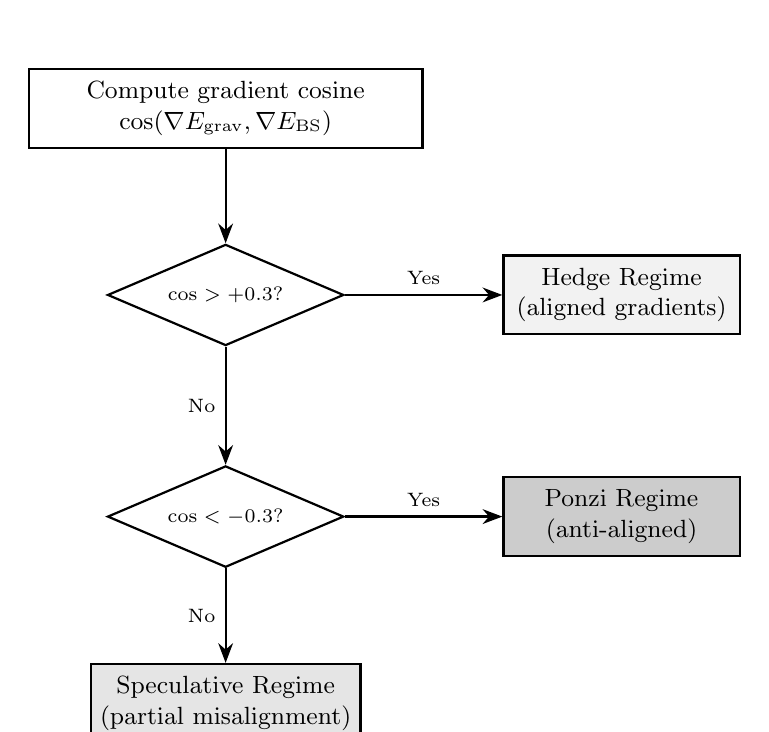
\begin{tikzpicture}[node distance=0.8cm]

\node[blk, minimum width=5cm] (grads) {Compute gradient cosine\\$\cos(\nabla E_{\mathrm{grav}}, \nabla E_{\mathrm{BS}})$};

\node[diam, below=1.2cm of grads, minimum width=3cm] (d1) {$\cos > +0.3$?};
\node[diam, below=1.5cm of d1, minimum width=3cm] (d2) {$\cos < -0.3$?};

\node[blk, right=2cm of d1, minimum width=3cm, fill=black!5] (hedge) {Hedge Regime\\(aligned gradients)};
\node[blk, right=2cm of d2, minimum width=3cm, fill=black!20] (ponzi) {Ponzi Regime\\(anti-aligned)};
\node[blk, below=1.2cm of d2, minimum width=3cm, fill=black!10] (specR) {Speculative Regime\\(partial misalignment)};

\draw[arr] (grads) -- (d1);
\draw[arr] (d1) -- node[above,font=\scriptsize]{Yes} (hedge);
\draw[arr] (d1) -- node[left,font=\scriptsize]{No} (d2);
\draw[arr] (d2) -- node[above,font=\scriptsize]{Yes} (ponzi);
\draw[arr] (d2) -- node[left,font=\scriptsize]{No} (specR);

\end{tikzpicture}
\end{center}

\newpage

%% =========  FIGURE 15  =========
\begin{center}
\textbf{Figure 15 --- Shared Adaptive Damping Function}
\end{center}

\begin{center}
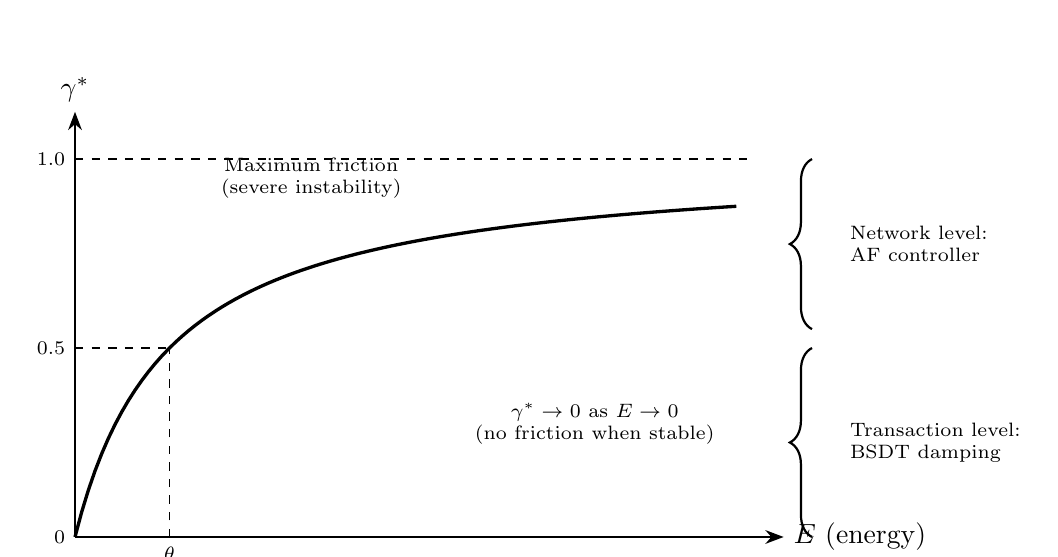
\begin{tikzpicture}[scale=1.2]

% Axes
\draw[thick, -{Stealth}] (0,0) -- (7.5,0) node[right] {$E$ (energy)};
\draw[thick, -{Stealth}] (0,0) -- (0,4.5) node[above] {$\gamma^*$};

% Curve
\draw[very thick, domain=0:7, samples=100] plot (\x, {4*\x/(\x+1)});

% Axis labels
\draw[dashed, thin] (0,4) -- (7.2,4);
\node[left, font=\scriptsize] at (0,4) {1.0};
\node[left, font=\scriptsize] at (0,2) {0.5};
\node[left, font=\scriptsize] at (0,0) {0};
\draw[dashed, thin] (0,2) -- (1,2);
\draw[dashed, thin] (1,0) -- (1,2);
\node[below, font=\scriptsize] at (1,0) {$\theta$};

% Annotations
\node[font=\scriptsize, align=center] at (2.5, 3.8)
  {Maximum friction\\(severe instability)};
\node[font=\scriptsize, align=center] at (5.5, 1.2)
  {$\gamma^* \to 0$ as $E \to 0$\\(no friction when stable)};

% Two-level annotation
\draw[thick, decorate, decoration={brace, amplitude=8pt}]
  (7.8, 0) -- (7.8, 2)
  node[midway, right=10pt, font=\scriptsize, align=left]
  {Transaction level:\\BSDT damping};
\draw[thick, decorate, decoration={brace, amplitude=8pt}]
  (7.8, 2.2) -- (7.8, 4)
  node[midway, right=10pt, font=\scriptsize, align=left]
  {Network level:\\AF controller};

\end{tikzpicture}
\end{center}

\vspace{1em}

\noindent The adaptive damping function $\gamma^*(E) = E/(E+\theta)$ operates at two levels:
\begin{itemize}
\item \textbf{Transaction level (BSDT):} modulates correction operator
intensity based on per-transaction blind-spot energy.
\item \textbf{Network level (Adaptive Friction):} drives enforcement
profile selection based on aggregate systemic energy.
\end{itemize}

\newpage

%% =========  FIGURE 16 (BONUS)  =========
\begin{center}
\textbf{Figure 16 --- Smart Contract Architecture}
\end{center}

\begin{center}
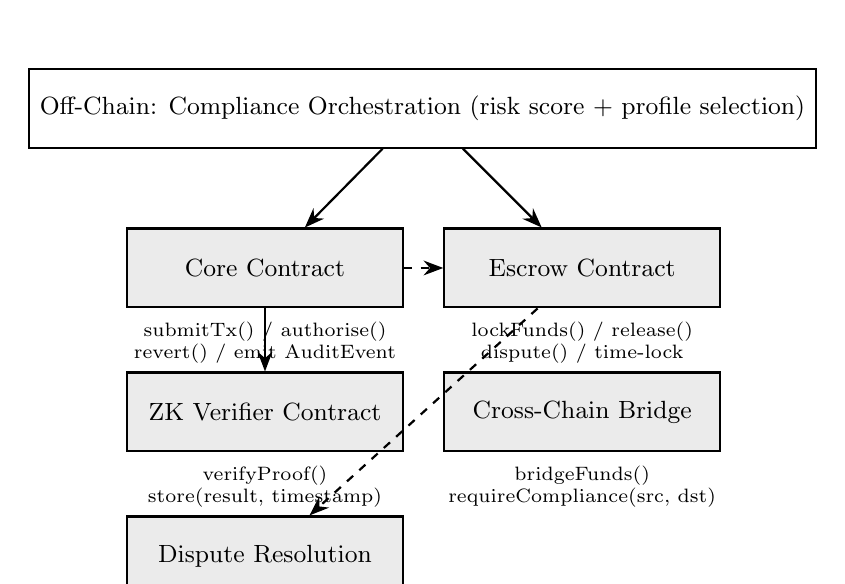
\begin{tikzpicture}[node distance=0.6cm]

\node[blk, minimum width=10cm] (offchain)
  {Off-Chain: Compliance Orchestration (risk score + profile selection)};

\node[blk, below=1cm of offchain, minimum width=3.5cm, fill=black!8, xshift=-2cm]
  (coreS) {Core Contract};
\node[blk, right=0.5cm of coreS, minimum width=3.5cm, fill=black!8]
  (escrowS) {Escrow Contract};

\node[blk, below=0.8cm of coreS, minimum width=3.5cm, fill=black!8]
  (zkverS) {ZK Verifier Contract};
\node[blk, right=0.5cm of zkverS, minimum width=3.5cm, fill=black!8]
  (bridgeS) {Cross-Chain Bridge};

\node[blk, below=0.8cm of zkverS, minimum width=3.5cm, fill=black!8]
  (disputeS) {Dispute Resolution};

% Function labels
\node[font=\scriptsize, below=0.05cm of coreS, anchor=north, align=center]
  {submitTx() / authorise()\\revert() / emit AuditEvent};
\node[font=\scriptsize, below=0.05cm of escrowS, anchor=north, align=center]
  {lockFunds() / release()\\dispute() / time-lock};
\node[font=\scriptsize, below=0.05cm of zkverS, anchor=north, align=center]
  {verifyProof()\\store(result, timestamp)};
\node[font=\scriptsize, below=0.05cm of bridgeS, anchor=north, align=center]
  {bridgeFunds()\\requireCompliance(src, dst)};

\draw[arr] (offchain) -- (coreS);
\draw[arr] (offchain) -- (escrowS);
\draw[arr] (coreS) -- (zkverS);
\draw[darr] (coreS) -- (escrowS);
\draw[darr] (escrowS) -- (disputeS);

\end{tikzpicture}
\end{center}

\end{document}
